The roadmap of approaches for achieving exactly-once is shown in Figure~\ref{roadmap}. White bricks show the paths, which are used by state-of-the-art stream processing systems. Unfortunately, all these approaches have high latency overhead. Working set snapshotting requires frequent blocking accesses to persistent storage. Atomic snapshotting and releasing make latency dependent on the time between snapshots. Micro-batching approaches experience high latency, because of the buffering on input.    

\begin{figure*}[htbp]
  \centering
  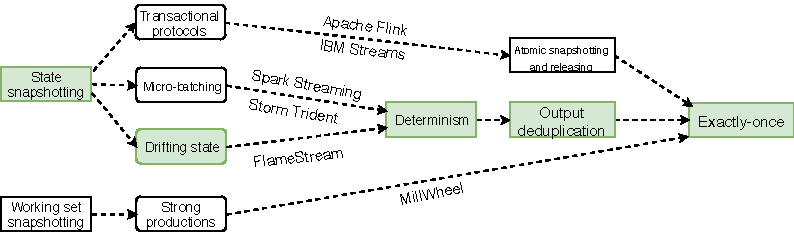
\includegraphics[width=0.97\textwidth]{pics/roadmap}
  \caption{The roadmap of approaches for achieving exactly-once guarantee. Green elements indicate the path for our approach}
  \label {roadmap}
\end{figure*} 

To the best of our knowledge, only micro-batching systems apply determinism for achieving exactly-once. It is commonly assumed that it is extremely hard to make stream processing system deterministic without high latency overhead. One reason behind this fact is that in general, Spark Streaming provides higher latency than pure streaming engines, e.g., Flink~\cite{karimov2018benchmarking}. However, in~\cite{we2018adbis} there was proposed a model called {\em drifting state} that allows achieving both determinism and low latency. Therefore, the open questions are: is it more efficient in practice to handle non-determinism by atomic snapshotting and releasing than to maintain a fair determinism in order to get exactly once? Can the green path provide lower latency than the most efficient white?